\documentclass{report}
\usepackage[margin=3cm]{geometry}
%\usepackage[landscape]{geometry}
\usepackage{longtable}
\usepackage{tabularx}
\usepackage[inline]{enumitem}
\usepackage[usenames,dvipsnames,svgnames,table]{xcolor}
\definecolor{light-gray}{gray}{0.80}
\usepackage{tikz}
\usetikzlibrary{calc,shapes, positioning,arrows}

\usepackage{minted}
\usepackage{listings}
\newcommand{\mi}[1]{\lstinline{#1}}

\makeatletter
\newenvironment{python}{%
  \VerbatimEnvironment
  \minted@resetoptions
  \setkeys{minted@opt}{}
      \begin{VerbatimOut}{\jobname.pyg}}
{%
      \end{VerbatimOut}
      \minted@pygmentize{python}
      \DeleteFile{\jobname.pyg}}
\makeatother

\usepackage{multicol}

\usepackage[ampersand]{easylist}
\setcounter{secnumdepth}{3}
\setcounter{tocdepth}{3}

\usepackage{bibleref}
\def\bv{\bibleverse}
\usepackage{ecjhebrew}
\newcommand{\cl}[2]{\begingroup\beginL\begingroup\color{#1}\beginR#2\endR\endgroup\endL\endgroup}
\newcommand{\hebr}[1]{\cjRL{#1}}

%\usepackage[usenames, dvipsnames]{color}
%\newcommand{\fixme}[1]{{#1}}

\title{Encoding options}
\author{Grietje Commelin}

\begin{document}
\maketitle


\section{Options for encoding a participant}

In analyzing participant references, it is important to distinguish between \\
\begin{enumerate*}[label=\itshape\alph*\upshape)]
\item the type of the reference / designation, and \\
\item the position of the reference in the clause.
\end{enumerate*}

\subsection{Types of reference}
In Biblical Hebrew, there are various options to refer to a participant. Some of these options are more extensive than others.

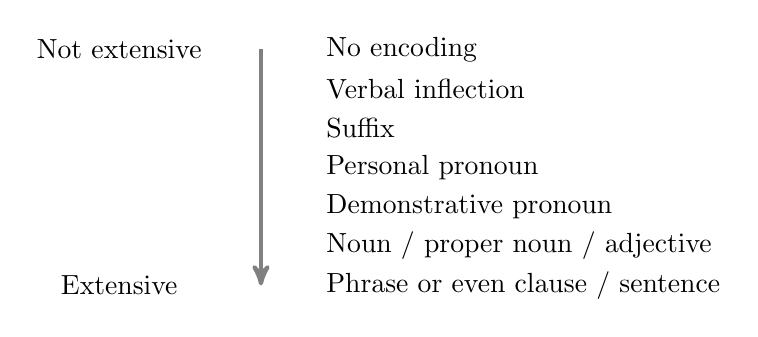
\begin{tikzpicture}[outline/.style={draw=#1,thick,fill=#1!50},
>=stealth',thick,black!50,text=black,
every new ->/.style={shorten >=.3cm}]
\draw  [->] (1.8,3) -- (1.8,0)[line width=1.5];
\node at (0,3){Not extensive};
\node at (0,0){Extensive};
\node at (2.5,3)[right]{No encoding};
\node at (2.5,2.5)[right]{Verbal inflection};
\node at (2.5,2)[right]{Suffix};
\node at (2.5,1.5)[right]{Personal pronoun};
\node at (2.5,1)[right]{Demonstrative pronoun};
\node at (2.5,0.5)[right]{Noun / proper noun / adjective};
\node at (2.5,0)[right]{Phrase or even clause / sentence};
\end{tikzpicture}

\subsubsection{Slots and sub-participants}
Usually, a sentence has a verb that takes certain elements with it: a subject, sometimes an object, or an indirect object. The verb \hebr{NTN} (``to give''), for example, needs a giver, a receiver and a gift. There can also be `free' optional elements, like a time reference or some other circumstantial information. The places where all these elements can occur, are called `slots'. Participant references occur on these slots.

Extensive references can sometimes be `deconstructed' into multiple sub-participants. This is the case, for example, with personal pronouns indicating a possessive relation: the phrase ``his father'' contains a reference to a father, but also to his son. Other examples are words with a \mi{sub_phrase} attached to them, such as ``\emph{fruit} trees \emph{bearing fruit after their kind, with their seeds in it, on the earth}''. This kind of references is dealt with on multiple levels: the reference as a whole is treated as such, but the sub-participants are also taken into account, because they fulfill a function in the text and influence other participant references.

A working hypothesis is that all potential participants that do not independently fulfill a slot in the text, are sub-participants. If there are multiple parallel participants in a subject slot, for example, these are not sub-participants but multiple independent participants. But if a participant reference carries with it an extensive clause that further specifies the reference \emph{without filling a slot itself}, the potential references within this \mi{clause} are considered sub-participants.

In order to make our data and analyses as clear as possible, we distinguish between various types of sub-participants. We do this by assigning them a value on the feature \mi{Sub} in \mi{gcdata.pt}:
\begin{itemize}
\item Value \mi{No} for a simple independent participant
\item Value \mi{Super} for an extensive independent participant reference that is deconstructed into sub-participants
\item Value \mi{Sub1} for the sub-participant with the same identity as the \mi{Super} participant it is part of; in other words the core of the extensive participant (e.g. ``his \emph{father}'')
\item Value \mi{Rec} for sub-participants with an identity different from the reference they are part of, and who either are a suffix on the \mi{Sub1} or are annotated with the \mi{Regens-rectum} relationship (e.g. ``\emph{his} father''). These are closely connected to the \mi{Sub1} participant.
\item Value \mi{RecPre} for sub-participants who precede the \mi{Sub1} sub-participant, and having an identity different from the reference they are part of (in other words, this is a \mi{Rec}sub-participant that does not follow but precede its \mi{parent}.) The typical example here is \hebr{KL}.
\item Value \mi{Attr} for sub-participants in clauses with the value \mi{Attr} on the feature \mi{Rela} in the ETCBC database. These usually provide extra information about a participant, without a different participant being involved in the description.
\end{itemize}

In complex cases, such as a \mi{Regens-rectum} relationship within an attributive clause, these labels can be nested.
In order to avoid unclarity in nested labels, sometimes the `empty' label \mi{0} is used. In this way we can differentiate, for example, between a word that is in a \mi{Rec} relationship to the corresponding \mi{Sub1} and a participant that is part of a larger \mi{Rec} clause without being in a \mi{Rec} relationship itself. The former has the simple label \mi{Rec}, the second is annotated with \mi{Rec 0}. A typical example is a circumstantial phrase within an attributive clause, such as a place reference introduced by a preposition.

\textbf{Is this 0 a good idea?? Also: need to think about imperative with object suffix (``subdue her'').}
\textbf{Think about constructions like \hebr{>RY KN<N}. Is \hebr{KN<N} Attr or Rec?}
\textbf{There are inconsistencies in the coding of suffixes attached to Sub1. Is this case `Sub1 Rec' or just `Rec'? Mainly in larger constructions}

In the case of a suffix, the labeling is altered a bit in order to avoid clumsy constructions in which the whole word has a \mi{Super} label, and is then splitted into the word without suffix and the suffix, with a \mi{Sub1} and \mi{Rec} label respectively. If the only difference between a \mi{Super} participant and its \mi{Sub1} is a suffix, the whole word is assigned a label \mi{Super1} (indicating this is a \mi{Super} participant which is almost identical with its \mi{Sub1}), and the suffix is coded as usual.

\paragraph{Types of participants: an example text}
Some examples of \mi{Rec} sub-participants are printed in blue in the text of \bibleverse{Gen}(3:18-20) below:\\

\noindent%
\begin{tabular}{rl}
\hebr{W QWY W DRDR TYMJX L\cl{green}{K}} & Thorns also and thistles will it bring forth to you;\\
\hebr{W >KLT >T <FB \cl{blue}{H FDH}} & and you will eat the herb \textcolor{blue}{of the field}. \\
\hebr{B Z<T \cl{blue}{>PJ}\cl{red}{K} T>KL LXM} & By the sweat \textcolor{blue}{of your face} will you eat bread \\
\hebr{<D CWB\cl{cyan}{K} >L H >DMH} & until you return to the ground, \\
\hebr{KJ MMNH LQXT} & for out of it you were taken. \\
\hebr{KJ <PR >TH} & For you are dust, \\
\hebr{W >L <PR TCWB} & and to dust you shall return. \\
\hebr{W JQR> H >DM CM \cl{blue}{>CT}\cl{red}{W} XWH} & The man called [the name \textcolor{blue}{of] his wife} Eve, \\
\hebr{KJ HW> HJTH >M \cl{blue}{KL XJ}} & because she was the mother \textcolor{blue}{of all living}. \\
\end{tabular}\\

In this text portion, we also see other participant references that deserve our attention. I marked them with red text color. These are suffixes on nouns and adjectives that fulfill a role comparable with the blue text portions (i.e. with \mi{sub_phrases} marked with the \mi{Regens-rectum} relationship). %The ETCBC database contains 18,476 of these suffixes.\\
As can be seen at the first line of Hebrew text, there are also suffixes on prepositions, that do not belong to this class. They independently fill a slot in the text, often that of a prepositional phrase. An example of this last category is marked with green in the text above. Still other options are subject or (indirect) object suffixes on verbs and participles. See an example in cyan above. These suffixes also fill a slot for themselves, and are not sub-participants.

\paragraph{Example of a labeled participant reference}
In \bibleverse{Gen}(1:28) we encounter the participant reference \hebr{KL XJH H RMFT <L H >RY}. This extensive reference can be deconstructed in the following way:
\begin{itemize}
\item \mi{Super} \hebr{KL XJH H RMFT <L H >RY}
\begin{itemize}
\item \mi{RecPre} \hebr{KL}
\item \mi{Sub1} \hebr{XJH}
\item \mi{Attr Super} \hebr{RMFT <L H >RY}
\begin{itemize}
\item \mi{Attr Sub1} \hebr{RMFT}
\item \mi{Attr 0} \hebr{>RY}
\end{itemize}
\end{itemize}
\end{itemize}

\bibleverse{Gen}(1:11) has an extensive reference about fruit trees: \hebr{<Y PRJ <FH PRJ L MNJW >CR ZR<W BW} -- ``fruit trees bearing fruit after their kind, with their seeds in it''.
\begin{tabbing}
\mi{Super} \hspace{20ex} \= \hebr{<Y PRJ <FH PRJ L MNJW >CR ZR<W BW} \\
\hspace{1ex} \mi{Sub1 Super} \> \hebr{<Y PRJ \cl{light-gray}{<FH PRJ L MNJW >CR ZR<W BW}} \\
\hspace{2ex} \mi{Sub1 Sub1} \> \hebr{<Y \cl{light-gray}{PRJ <FH PRJ L MNJW >CR ZR<W BW}}\\
\hspace{2ex} \mi{Sub1 Rec} \> \hebr{\cl{light-gray}{<Y} PRJ \cl{light-gray}{<FH PRJ L MNJW >CR ZR<W BW}}\\
\hspace{1ex} \mi{Attr Super} \> \hebr{\cl{light-gray}{<Y PRJ} <FH PRJ L MNJW >CR ZR<W BW} \\
\hspace{2ex} \mi{Attr Sub1} \> \hebr{\cl{light-gray}{<Y PRJ} <FH \cl{light-gray}{PRJ L MNJW >CR ZR<W BW}} \\
\hspace{2ex} \mi{Attr Rec Super} \> \hebr{\cl{light-gray}{<Y PRJ <FH} PRJ L MNJW >CR ZR<W BW} \\
\hspace{3ex} \mi{Attr Rec Sub1} \> \hebr{\cl{light-gray}{<Y PRJ <FH} PRJ \cl{light-gray}{L MNJW >CR ZR<W BW}} \\
\hspace{3ex} \mi{Attr Rec Attr Super1} \> \hebr{\cl{light-gray}{<Y PRJ <FH PRJ L} MNJW \cl{light-gray}{>CR ZR<W BW}} \\
\hspace{4ex} \mi{Attr Rec Attr Rec} \> \hebr{\cl{light-gray}{<Y PRJ <FH PRJ L MNJ}W \cl{light-gray}{>CR ZR<W BW}} \\
\hspace{3ex} \mi{Attr Rec Attr Super} \> \hebr{\cl{light-gray}{<Y PRJ <FH PRJ L MNJW} >CR ZR<W BW} \\
\hspace{4ex} \mi{Attr Rec Attr Super1} \> \hebr{\cl{light-gray}{<Y PRJ <FH PRJ L MNJW >CR} ZR<W \cl{light-gray}{BW}} \\
\hspace{5ex} \mi{Attr Rec Attr Rec} \> \hebr{\cl{light-gray}{<Y PRJ <FH PRJ L MNJW >CR ZR<}W \cl{light-gray}{BW}} \\
\hspace{4ex} \mi{Attr Rec Attr Rec} \> \hebr{\cl{light-gray}{<Y PRJ <FH PRJ L MNJW >CR ZR<W B}W} \\
\end{tabbing}



\subsubsection{Encoding options on various slots}
The options that are available for encoding a participant in a certain slot, are constrained by (among other things) grammatical features of the slot and its immediate textual context, such as a slot's role in the sentence.

How extensive this relevant context is, can vary. Sub-participants, for example, are dependent on their `parent', and not directly on \mi{clause_type} and \mi{phrase_function}. They are in a way embedded in an independent participant, and thereby isolated from the influence of other textual elements. They live within the protection of their family, and do not fill a slot themselves. My hypothesis is that (the clearest category of) these occurrences are annotated with the \mi{Regens-rectum} relationship in the ETCBC database.\\

In order to get an impression of the possibilities to express participant references on various slots, below is an overview of options that occur in direct speech sections of the Old Testament. The frequency of the various options does of course differ, and there are many other factors that are not taken into account here. But at least we can learn from \emph{missing} types of encoding that these apparently fall outside the range of available options.

\paragraph{Subject encoding}
\begin{itemize}
\item With (verbal) inflection: \bibleverse{Gen}(14:22) \\ \hebr{\cl{red}{HRJMTJ} JDJ >L JHWH >L <LJWN QNH CMJM W >RY} \\ ``I have lifted up my hand to Yahweh, God Most High, possessor of heaven and earth...''
\item With a suffix (on verb): \bibleverse{Gen}(2:17) \\ \hebr{B JWM \cl{red}{>KLK} MMNW MWT TMWT} \\``... in the day that you eat of it, you will surely die.''
\item With a suffix (on noun): \bibleverse{Gen}(20:7) \\ \hebr{>M \cl{red}{>JNK} MCJB D< KJ MWT TMWT} \\ ``If you don't restore her [= Sarah, GC], know for sure that you will die.''
\item With a personal pronoun: \bibleverse{Gen}(3:11) \\ \hebr{MJ HGJD LK KJ <JRM \cl{red}{>TH}} \\ ``Who told you that you were naked?''
\item With a demonstrative pronoun: \bibleverse{Gen}(2:23) \\ \hebr{\cl{red}{Z>T} H P<M <YM M <YMJ} \\ ``This is now bone of my bones...''
\item With an interrogative pronoun: \bibleverse{Gen}(3:11) \\ \hebr{\cl{red}{MJ} HGJD LK KJ <JRM >TH} \\ ``Who told you that you were naked?''
\item With a verb (participle): \bibleverse{Gen}(4:15) \\ \hebr{KL \cl{red}{HRG} QJN CB<TJM JQM} \\ ``Therefore whoever slays Cain, vengeance will be taken on him sevenfold.''
\item With a noun: \bibleverse{Gen}(2:18) \\ \hebr{L> VWB HJWT \cl{red}{H >DM} L BDW} \\ ``It is not good for the man to be alone.''
\item With a noun with suffix: \bibleverse{Gen}(4:6) \\ \hebr{LMH NPLW \cl{red}{PNJK}} \\ ``Why has (the expression of) your face fallen? [GC]''
\item With a personal noun: \bibleverse{Gen}(4:9) \\ \hebr{>J \cl{red}{HBL} >XJK} \\ ``Where is Abel, your brother?''
\item With an adjective: \bibleverse{Gen}(18:24) \\ \hebr{>WLJ JC XMCJM \cl{red}{YDJQM} B TWK H <JR} \\ ``What if there are fifty righteous within the city?''
\item With a phrase (multiple words): \bibleverse{Gen}(24:7)

\begin{cjhebrew}
\cl{red}{JHWH >LHJ H CMJM >CR LQXNJ M BJT >BJ W M >RY MWLDTJ W >CR DBR LJ W >CR NCB< LJ L >MR L ZR<K >TN >T H >RY H Z>T} \\
HW> JCLX ML>KW L PNJK
\end{cjhebrew}

``Yahweh, the God of heaven -- who took me from my father’s house, and from the land of my birth, who spoke to me, and who swore to me, saying, `I will give this land to your offspring' -- he will send his angel before you...''
\end{itemize}

\paragraph{Object encoding}
Objects are sometimes introduced by the nota objecti \hebr{>T}. These are dealt with in section \ref{prep}, because the ETCBC database sees \hebr{>T} as a preposition. Indirect objects are also introduced with a preposition. \textcolor{blue}{Always?} Objects without a preposition can be encoded in the following ways:
\begin{itemize}
\item With a suffix: \bibleverse{Gen}(6:7) \\ \hebr{NXMTJ KJ \cl{red}{<FJTM}} \\ ``I am sorry that I have made them.''
%\item With a personal pronoun: \bibleverse{}
\item With a demonstrative pronoun: \bibleverse{Gen}(3:14) \\ \hebr{KJ <FJT \cl{red}{Z>T} >RWR >TH M KL H BHMH} \\ ``Because you have done this, you are cursed above all livestock...''
\item With an interrogative pronoun: \bibleverse{Gen}(4:10) \\ \hebr{\cl{red}{MH} <FJT} \\ ``What have you done?''
\item With a verb (participle): \bibleverse{Gen}(23:11) \\ \hebr{QBR \cl{red}{MTK}} \\ ``Bury your dead.''
\item With a noun: \bibleverse{Gen}(1:26) \\ \hebr{N<FH \cl{red}{>DM} B YLMNW} \\ ``Let's make man in our image''
\item With a noun with suffix: \bibleverse{Gen}(13:14) \\ \hebr{F> N> \cl{red}{<JNJK}} \\ ``Now, lift up your eyes...''
\item With a personal noun: \bibleverse{Ex}(4:27) \\ \hebr{LK LQR>T \cl{red}{MCH} HMDBRH} \\ ``Go into the wilderness to meet Moses.''
\item With an adjective: \bibleverse{Gen}(3:22) \\ \hebr{HN H >DM HJH K >XD MMNW L D<T \cl{red}{VWB} W \cl{red}{R<W}} \\ ``Behold, the man has become like one of us, knowing good and evil.''
\item With a phrase (multiple words): \bibleverse{Gen}(1:11) \\ \hebr{TDC> H >RY DC> <FB MZRJ< ZR< \cl{red}{<Y PRJ <FH PRJ L MJNW >CR ZR<W BW} <L H >RY} \\ ``Let the earth yield grass, herbs yielding seeds, and fruit trees bearing fruit after their kind, with their seeds in it, on the earth.''
\end{itemize}

\paragraph{Encoding options after prepositions}\label{prep}
The Old Testament has many prepositions, usually followed by participant references. The option of encoding a participant by (verbal) inflection obviously is not available for prepositions, since these do not have inflection. They just serve as an introduction to a participant reference, and do not form part of the reference themselves. Except for inflection (and zero encoding), all options are available for prepositions, as will be shown with examples below.

\begin{itemize}
\item With a suffix: \bibleverse{Gen}(4:10) \\ \hebr{QWL DMY >XYK Y<QJM \cl{red}{>LJ} MN H>DMH} \\ ``Your brother's blood cries to me from the ground.''
\item With a personal pronoun: \bibleverse{Ex}(36:1) \\ \hebr{NTN JHWH XKMH WTBWNH \cl{red}{BHMH}} \\ ``... JHWH has put wisdom and understanding in them... [GC]''
\item With a demonstrative pronoun: \bibleverse{Gen}(2:23) \\ \hebr{\cl{red}{LZ>T} YQR> >CH} \\ ``She will be called `woman'... ''
\item With an interrogative pronoun:  \bibleverse{Gen}(15:8) \\ \hebr{>DNJ JHWH \cl{red}{B MH} >D< KJ >JRCNH} \\ ``Lord Yahweh, how will I know that I will inherit it?''
\item With a verb (participle): \bibleverse{Gen}(1:14) \\ \hebr{JHJ M>RT BRQJ< HCMJM \cl{red}{LHBDJL} BJN HJWM WBJN HLJLH} \\ ``Let there be lights in the expanse of the sky to divide the day from the night''
\item With (article and) noun: \bibleverse{Gen}(4:10) \\ \hebr{QWL DMY >XYK Y<QJM >LY \cl{red}{MN H>DMH}} \\ ``Your brother's blood cries to me from the ground.''
%\item With a noun with suffix: \bibleverse{Gen}(3:10) \\ \hebr{\cl{red}{>T QLK} CM<TJ B HGN} \\ ``I heard your voice in the garden...''
\item With a noun with suffix: \bibleverse{Gen}(3:14) \\ \hebr{<L \cl{red}{GXNK} TLK} \\ ``You shall go on your belly..''
\item With a personal noun: \bibleverse{Gen}(9:27) \\ \hebr{JPT >LHJM \cl{red}{LJPT}} \\ ``May God enlarge Japheth.''
\item With an adjective: \bibleverse{Gen}(18:23) \\ \hebr{H>P TSPH YDJQ \cl{red}{<M RC<}} \\ ``Will you consume the righteous with the wicked?''
\end{itemize}

\paragraph{Nota objecti \hebr{>T}}
A special category are the nota objecti \hebr{>T} and the nota accusativi \hebr{JT} (occurring only once, in \bibleverse{Dan}(3:12)). These introduce an object slot, and have the same options as other prepositions, except for the personal pronoun, which does not occur anywhere in the Old Testament.
\begin{itemize}
\item With a suffix: \bibleverse{Gen}(7:1) \\ \hebr{KJ \cl{red}{>TK} R>JTJ YDJQ} \\ ``I have seen your righteousness before me in this generation.''
\item With a demonstrative pronoun: \bibleverse{Gen}(29:33) \\ \hebr{KJ CM< JHWH KJ FNW>H >NKJ W JTN LJ GM \cl{red}{>T ZH}} \\ ``Because Yahweh has heard that I am hated, he has therefore given me this son also.''
\item With an interrogative pronoun: \bibleverse{IIKings}(19:22) \\ \hebr{\cl{red}{>T MJ} XRPT} \\  ``Whom have you defied?''
\item With a verb (participle): \bibleverse{Gen}(23:6) \\ \hebr{B MBXR QBRJNW QBR \cl{red}{>T MTK}} \\ ``Bury your dead in the best of our tombs.''
\item With (article and) noun: \bibleverse{Gen}(4:12) \\ \hebr{T<BD \cl{red}{>T H>DMH}} \\ ``When you till the ground...''
\item With a noun with suffix: \bibleverse{Gen}(22:2) \\ \hebr{QX N> \cl{red}{>T BNK} >T JXJDK >CR >HBT >T JYXQ} \\ ``Now take your son, your only [son], whom you love, Isaac [GC]''
\item With a personal noun: \bibleverse{Gen}(22:2) \\ \hebr{QX N> >T BNK >T JXJDK >CR >HBT \cl{red}{>T JYXQ}} \\ ``Now take your son, your only [son], whom you love, Isaac [GC]''
\item With an adjective: \bibleverse{Gen}(22:2) \\ \hebr{QX N> >T BNK \cl{red}{>T JXJDK} >CR >HBT >T JYXQ} \\ ``Now take your son, your only [son], whom you love, Isaac [GC]''
\end{itemize}
These options can be extended by \mi{subphrases} or elaborate descriptions of the object, thus creating an extensive participant reference. The reference to \bibleverse{Gen}(22:2) can serve as an example here.

\paragraph{\mi{Rec} sub-participants}
Sub-participants annotated with the \mi{rectum} part of the \mi{Regens-rectum relation} are, as we have seen above, not directly dependent on the grammatical context beyond the word that reigns them. We therefore consider words annotated as \mi{Regens} as a separate category of introduction, followed by an alternative `slot'. Since this relationship only occurs on words, it is not assigned to suffixes. However, I think there are suffixes fulfilling a comparable function:

\begin{itemize}
\item With a suffix: \bibleverse{Gen}(1:11) \\ \hebr{<Y PRJ <FH PRJ L MJN\cl{red}{W}} \\ ``(...) fruit trees bearing fruit after their kind''
\end{itemize}

Demonstrative pronouns often occur immediately after a noun, and then refer back to it without a change in identity. The same can happen with personal pronouns and adjectives, although adjectives with a different identity also occur. All these options, of which examples are given below, are more comparable to the article than to the sort of possessive relationship that is reflected by the \mi{rectum} elements with an identity different from that of the \mi{Regens}. They elaborate further on the last mentioned participant, giving more specific information, without referencing to other participants in this description.

\begin{itemize}
%\item With (verbal) inflection: \bibleverse{Gen}
\item With a personal pronoun: \bibleverse{Deut}(13:4) \\ \hebr{L> TCM< >L DBRJ HNBJ> \cl{red}{HHW>}} \\ ``(...) you shall not listen to the words of that prophet''
\item With a demonstrative pronoun: \bibleverse{Gen}(21:10) \\ \hebr{GRC H >MH \cl{red}{H Z>T} W >T BNH} \\ ``Cast out this servant and her son!'' \footnote{Found as \mi{rec}, but annotated with \mi{dem}}
\item With an adjective (same identity): \bibleverse{Gen}(1:20) \\ \hebr{JCRYW H MJM CRY NPC \cl{red}{XJH}} \\ ``Let the waters abound with living creatures''
\end{itemize}

Examples of references with a different identity:
\begin{itemize}
\item With a demonstrative pronoun: \textbf{????} \bibleverse{Ex}(13:8) \\ \hebr{B <BWR \cl{red}{ZH} <FH JHWH LJ B Y>TJ M MYRJM} \\ ``It is because of that which Yahweh did for me when I came out of Egypt.''
\item With an interrogative pronoun: \footnote{Found as \mi{status constructus} followed by \mi{prin}; not indicated by \mi{rec}} \bibleverse{Gen}(24:23) \\ \hebr{BT \cl{red}{MJ} >T} \\ ``Whose daughter are you?''
\item With a verb (participle): \bibleverse{Gen}(22:17) \\ \hebr{W JRC ZR<K >T C<R \cl{red}{>JBJW}} \\ ``(...) and your offspring will possess the gate of his enemies [GC]''
\item With a noun: \bibleverse{Gen}(1:20) \\ \hebr{<WP J<WPP <L H >RY <L PNJ RQJ< \cl{red}{H CMJM}} \\ ``(...) let birds fly above the earth in the open expanse of the sky''
\item With a personal noun: \bibleverse{Gen}(9:26) \\ \hebr{BRWK JHWH >LHJ \cl{red}{CM}} \\ ``Blessed be Yahweh, the God of Shem''
\item With an adjective (different identity): \bibleverse{Ex}(23:8) \\ \hebr{DBRJ \cl{red}{YDJQJM}} \\ ``(...) the words of the righteous''
\item With a phrase (multiple words): \bibleverse{Gen}(3:2) \\ \hebr{M PRJ \cl{red}{<Y H GN} N>KL} \\ ``We may eat from the fruit of the trees of the garden [GC]''
\end{itemize}

\paragraph{Summary of the available encoding options}
. \\
%\noindent%
\begin{tabularx}{\textwidth}{|l|X|X|X|X|X|X|}
\hline
\emph{Available encoding options} & \emph{Subject} & \emph{Object} & \emph{On prepositions} & \cjRL{>T} & \emph{Sub-participants (Rec)} \\ \hline
\emph{Verbal inflection} & Yes & No & No & No & No \\ \hline
\emph{Suffix} & Yes & Yes & Yes & Yes & Yes (comparable) \\ \hline
\emph{Personal pronoun} & Yes & No & Yes & No & Yes (same identity) \\ \hline
\emph{Demonstrative pronoun} & Yes & Yes & Yes & Yes & Yes (at least with same identity)\\ \hline
\emph{Interrogative pronoun} & Yes & Yes & Yes & Yes & Yes \\ \hline
\emph{Verb (participle)} & Yes & Yes & Yes & Yes & Yes \\ \hline
\emph{Noun} & Yes & Yes & Yes & Yes & Yes \\ \hline
\emph{Personal noun} & Yes & Yes & Yes & Yes & Yes \\ \hline
\emph{Adjective} & Yes & Yes & Yes & Yes & Yes \\ \hline
\emph{Phrase} & Yes & Yes & Yes & Yes & Yes \\ \hline
\end{tabularx}

\subsection{Position of references}
Not only the encoding type of the reference, but also its place in the clause or sentence can be important. Some references are bound to a fixed position within the clause. Verbal inflection, of course, manifests on the verb. Suffixes are attached to nouns, verbs et cetera. Extensive references are more flexible with regard to their position. This leaves some options open; the difference between a \mi{We-X-Qatal} and \mi{We-Qatal-X clause}, for example, only is the relative position of the verb and the subject. Since the ordering of verb and participant reference thus is not fully determined by verb type and reference type, we need to reckon with the possibility of meaningful decisions based on different factors here.

\subsection{Prominence}
As we saw above, participants can be encoded more or less extensively. In general, extensive encodings draw more attention, and thus are more prominent in a text, than less extensive ones. However, prominence is not only dependent on the encoding option chosen, but also on its textual context.\\
On the one hand, the grammatical context limits the range of encoding options from which an author can choose. The clause type in which a reference occurs, its grammatical function within the clause, and other factors influence the range of options that are available. Some of these factors are yet unclear, or not easily circumscribed in computer code. Therefore I start with the factors that are indisputable, and try to find others in a process of thinking, testing and rethinking. This is all about the prominence of a reference relative to the grammatical options available.\\
On the other hand, the prominence as perceived by readers is also dependent on neighboring references, the number of active participants, and many other things that are not easily caught in grammatical rules. These factors will get our attention later on.

Proposal for indicating prominence:
\begin{itemize}
\item 0 is reserved for `no reference at all'
\item 1 is for verbal inflection
\item 2 is for suffixes
\item 3 is for the personal pronouns
\item 4 is for the demonstrative pronouns
\item 5 is for the noun (\mi{subs}), proper noun (\mi{nmpr}) and adjective (\mi{adjv})
\item 6 is reserved for phrases etc, so noun+
\end{itemize}

\section{The chicken or the egg}
The encoding of participant references is only one feature among many in a text. For example, a text also has certain clause types, phrase types, verb types, et cetera.
An important question is the order in which textual choices on different aspects were made by authors and editors of our text corpus. In other words: which features are chosen first, and how do they constrain the liberty of choice of other features?
To give a concrete example, we consider \bibleverse{Genesis}(3:5): \textbf{To fix: insert Hebrew text!}

The serpent tells the woman that, if eating from the forbidden fruit, she will not die. It then continues stating that ``God knows that\ldots'' something very different will happen. This `knowing' of God is expressed by a participle. Since participles do not show a person (they do show number and gender), expressing person by something like verbal inflection is no option here. The range of choices is limited by the chosen \mi{clause_type} -- if we assume that the clause type was chosen first.

We can also imagine the process to go the other way round: an author wants to use a particular participant reference, and chooses a clause type that fits his requirements.
A third possibility, probably closer to the truth, is that the choices of both clause type and participant reference are (more or less unconsciously) based on still other factors like the larger structure of a text. Participants do not occur independently from a text structure, they form a key part of it. In other words, we do not have a chicken and an egg but two little chickens growing up together.

This discussion might seem a bit hypothetical, but it is important for the meaning we assign to participant reference types. After all, if the author did not have any choice, we can not assign meaning to his decision. If, however, he deliberately chose to write a certain encoding, he probably had good reason to do so -- and we want to know what that reason was.

\subsection{Flow chart for interpreting texts}
We will probably never know for sure how exactly these processes worked in an author's head. And we surely cannot ask him anymore. But we can analyze the resulting texts and assign meaning to the phenomena we encounter. My hypothesis is that \mi{clause_types} are among the clearest expressions of the text structure, while `reading' this structure from participant references is a little more complicated because there are more factors in play. Moreover, given a certain range of options, it is easier to assign a ranking to participant encodings than to \mi{clause_types}. This makes it more logical to take \mi{clause_types} and \mi{phrase_functions} as a starting point, and see which encoding types are used on the various `slots' in the Old Testament.\\
For sub-participants, this does not make sense. They are dependent on their `parent', and not directly on \mi{clause_type} and \mi{phrase_function}.


\subsection{Stuff that should not be forgotten}
The types (\mi{F.etcbc4\_ft\_typ.v(node)}) of \mi{clauses} and \mi{clause_atoms} are identical. Same for \mi{phrase} and \mi{phrase_type}.

Lettinga 25d:
\begin{itemize}
\item Accusativus wordt, wanneer deze bepaald is, in proza gewoonlijk aangegeven door \hebr{>T}.
\item Indirect object (dativus) door \hebr{L}
\item Genitivus ook vaak met \hebr{L}
\item Vocativus vaak met lidwoord, maar niet bij eigennamen
\end{itemize}

Indirect (?) object with suffix on verb: Gen 3:13

I annotated MJM as individual; is this correct?

%Noun, Noun\_phrase, Name, Name\_phrase, Pers\_pronoun, Other\_pronoun, Suffix, Verb

\end{document}

